\chapter{Benchmarks and Discussion}

We will present a number of benchmarks designed to compare and
quantify the differences in performance of the parallelization models
that we have implemented.

Since the execution time is only dependent on the total amount of work
that a network performs and not how the processes in the network are
connected, all of our benchmarks will use a ring-shaped
(\cref{fig:benchnetwork}) network with the participating processes
performing varying amounts of work.

We conjecture that the scalability of our implementation will depend
strongly on the nature of the workload performed by the SME-networks
benchmarked. We will therefore benchmark both light and heavy

As our previously presented hypotheses states, we expect our
benchmarks to show that the effects of syncing becomes more pronounced
as we decrease the amount of work performed by our processes while it,
on the other hand, will become amortized as the amount of work
performed by each process increases.

\begin{figure}
\centering
\includegraphics{figures/ring}
\caption[SME network used for benchmarking]{Illustration showing the
  layout of the network used for benchmarking. The blue circles
  represents processes and the arrows represents busses}
\label{fig:benchnetwork}
\end{figure}


\section{Testing methodology}
All of the time measurements shown were performed inside the SME
framework itself using the C++11 \texttt{<chrono>} functions, and
measures only the actual execution time of the network. It therefore
does not include the constant time required to generate the
benchmarked networks. Two different hardware platforms has been used
for performing the benchmarks: One AMD and one Intel platform.

The Intel machine has the following specs
\begin{itemize}
\item CPU: Intel Xeon E3-1245 V2 @ 3.40GHz
\item RAM: 32GB
\item OS: Linux
\end{itemize}

and the AMD machines used are part of the eScience cluster at NBI and
boasts the following specs:
\begin{itemize}
  \item CPU: AMD...
  \item RAM: 128GB
  \end{itemize}

Since the instruction set used by the two CPU's support incompatible
optimizationns, code generated for one will not run unmodified on the
other. Therefore, code executed on the AMD CPU were compiled with the
GCC flags \texttt{-mtune=barcelona -march=barcelona}, while code
executed on the Intel CPU were compiled with \texttt{-march=native} on
a Core i7 machine. GCC 4.9 was used in both cases. Furthermore,
due to incompatible versions of libstdc++ on the test machines, all
benchmarks has been performed using statically linked binaries.

All of the benchmarks has been executed 5 times and the graphs are
based on the averages of these. Error bars showing the minimum and
maximum deviation from the average has been added to all graphs,
however, in some cases the deviations benchmark runs were too small
for the error bars to be visible.

We calculate our speedup using the formula

\begin{equation*}
S = \frac{T_{\text{old}}}{T_{\text{new}}}
\end{equation*}

where $S$ is the achieved speedup, $T_{\text{old}}$ is the original
(pre-improvement) speed and $T_{\text{new}}$ is the new
(post-improvement) speed \cite{hennessy2012computer}.

The raw benchmark data can be found in \cref{chap:benchdata}.

\section{Synchronization dominated}
In this section, we present a benchmark, where the performance is
predominantly determined by the efficiency of the synchronization
mechanisms.

We perform this benchmark, by creating a ring which does nothing other
than passing an integer value from process to process. Sine each
process only takes a few clock cycles to execute, we expect that this
benchmark will reveal the overhead caused by synchronization.

urthermore, since we actually 
e

The following source code used in the execution unit of the process
\begin{listing}{H}
\begin{minted}{C++}
void step() {
  int val = in->read();
  out->write(++val);
}
\end{minted}
\caption{Source code for the execution unit of the processes
  participating in the network used for sync-dominated benchmarking}
\end{listing}

\begin{figure}
\centering
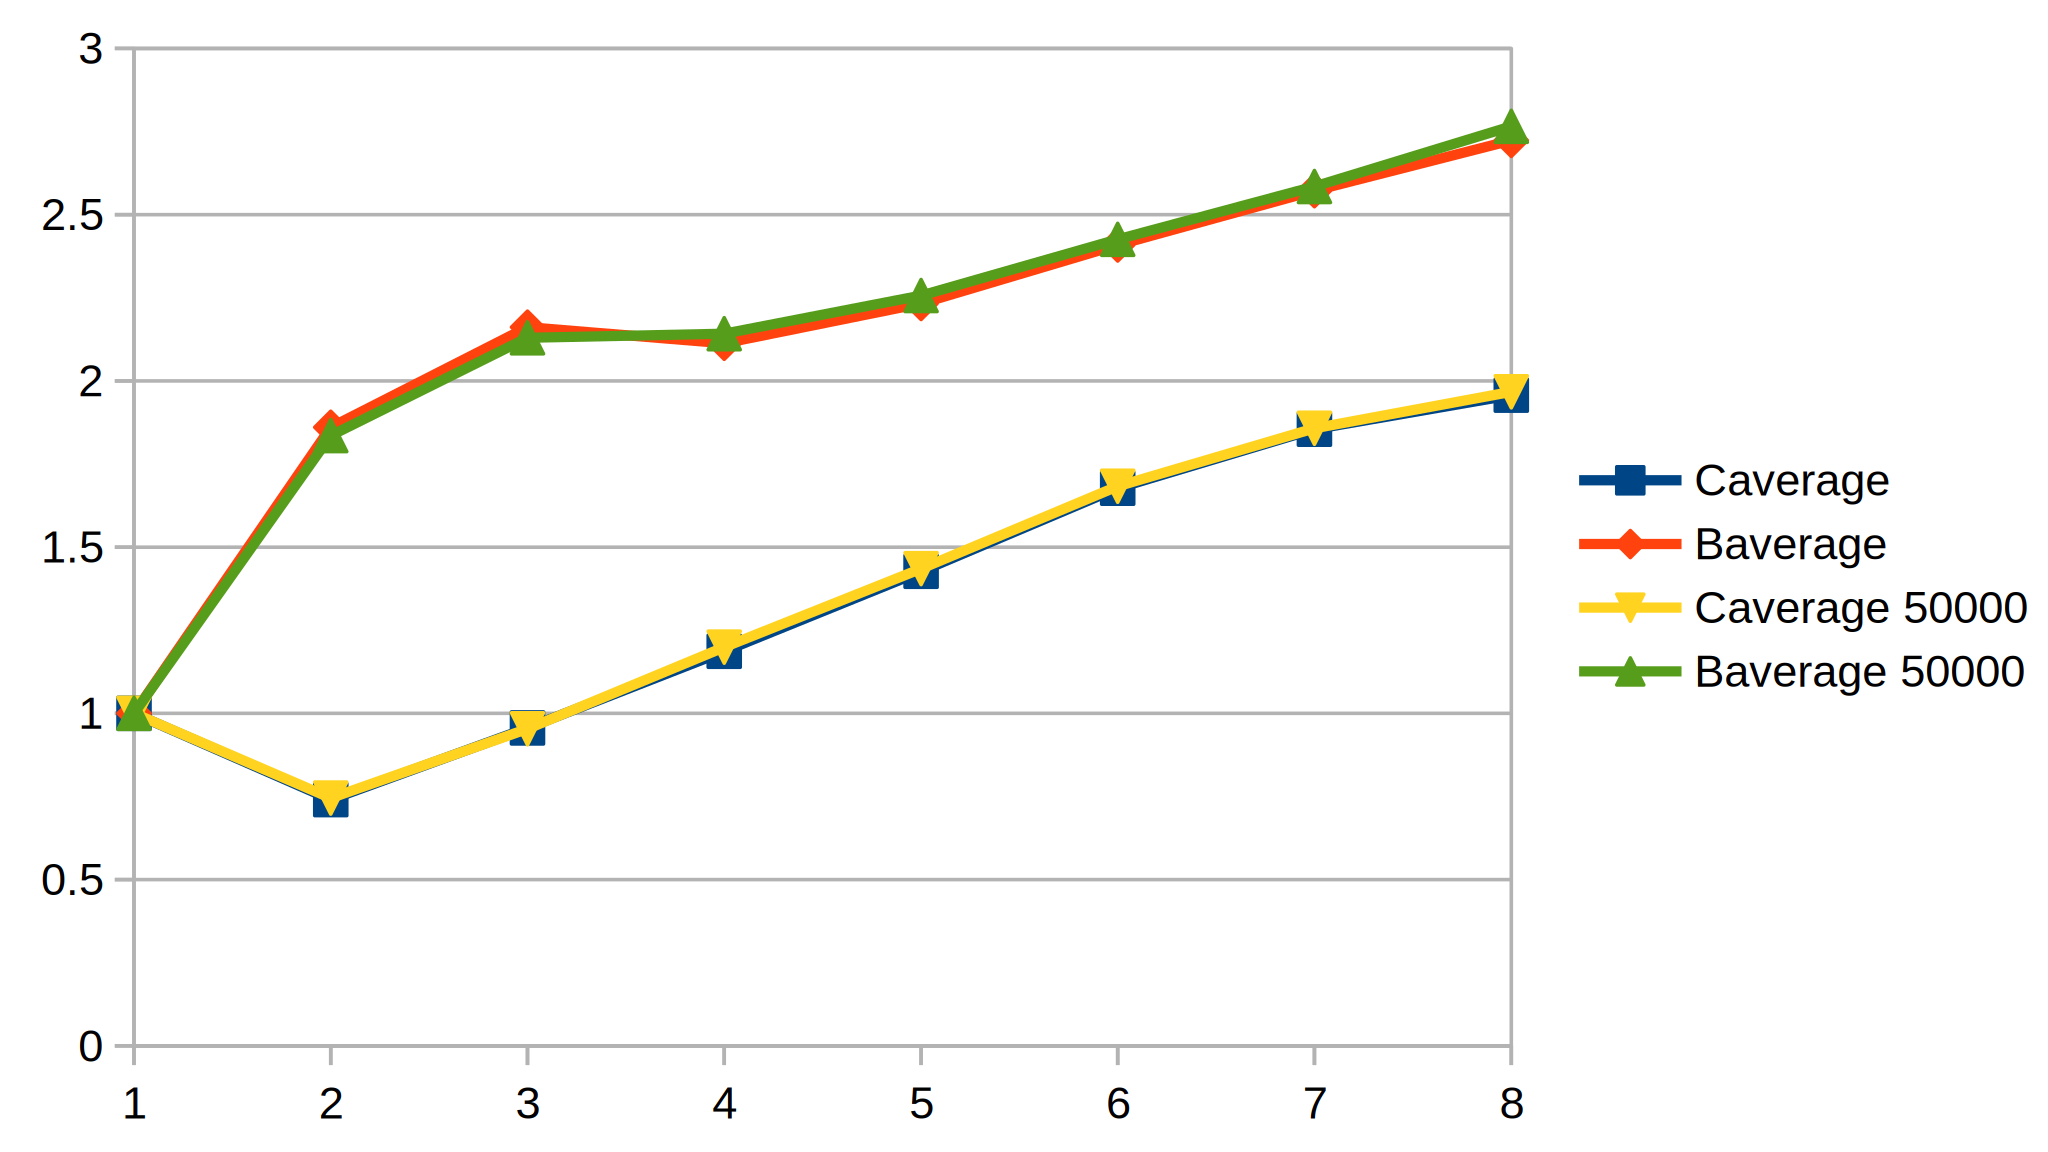
\includegraphics{graphs/graphone}
\caption[Benchmark graph]{Graph showing the speedup of a SME network
  consisting of 20000 and 50000 processes respectively when executed
  for 50000 cycles on an Intel Xeon CPU}
\label{fig:intel-sync}
\end{figure}

\begin{figure}
\centering
\includegraphics{graphs/amd-sync-20000}
\caption[Synchronization-dominated benchmark on AMD cluster]{Benchmark results for a network of 20000 processes running
for 100000 iterations on the AMD cluster}
\label{fig:amd-sync}
\end{figure}


\subsection{Discussion}
We can observe a number of things from the results that can bee seen
in \cref{fig:intel-sync}.  This benchmarks shows the performance of
two different networks, one with 20000 processes and one with 50000
processes. Both networks executed 100000 cycles.

When looking at the graph for our worker-queue model, One thing that
is clearly visible from this benchmark is the overhead produced by the
atomic increment that is required.. This model is doubly penalized
when running the benchmark since we, addition to then time required by
the atomic increment, also need to wait for all of the threads to sync
up at the end of a cycle. What is slightly surprising, however, is the
actual performance that this method shows. It performs significantly
worse when going from one to two threads. The most likely explanation
for this result is CPU optimizations which make atomic updates of a
variable less costly when these updates only occures from one thread.

Our static orchestration model performs quite decently and produces
almost 2x speedup when going from 1 to 2 threads. When adding
additional threads, the speedup decreases, which is expected since the
time spent synchronizing is increased, \fxnote{which manifests as
  dropping CPU-utilization. When running 4 threads, the CPU
  utilization drops to 360\%, unfortunately, I probably wont have time
  to measure or show this}

Common for both of the models, is that the size of the network
executed seems to have no impact on the relative speedups achieved.

Since the Xeon CPU that the benchmarks were performed on only have 4
cores with Hyper Threading, another interesting observation is that
Hyper Threading seems to give a significant additional speedup. One
hypothesis for explaining the cause of this is that branch-prediction
isn't very effective at predicting which functions we're going to call
in our SME network. A branch mis-prediction causes the CPU-pipeline to
be cleared, creating an optimal condition for Hyper Threading to make
use of the empty pipeline-stages\cite{fog2014microarchitecture} While
branch-predictors This hypothesis could be tested by running the
program through a profiler in order to measure the number of
mis-predictions occurring. At this time, these results are not
available.

\Cref{fig:amd-sync} show the results of the smallest version of the
benchmark running on the AMD cluster. The results are significant
worse compared to the results of the Intel Xeon CPU, both in absolute
running times \fxnote{Is it OK to show the numbers?} and
speedup. Early possible explanations was that, due to the extremely
long running time of the benchmark, we were seeing the effects of the
process being moved between CPU-cores. However, the results remained
the same after pinning the threads to CPU-cores placed on the same
NUMA-unit. Thus, the only reasonable explanation explanation is that our
syncronization mechanisms is significantly less optimized on the AMD
CPU compared to the Intel CPU.

Another thing standing out from this benchmark is the huge variability
between the different benchmark runs as shown by the Y-axis error bars.

Due to these very poor initial benchmark results, we didn't attempt
benchmark the synchronization dominated network with different problem
sizes on the AMD-cpu.


\section{Cycle dominated}

\begin{figure}
\centering
\includegraphics{graphs/heavy-ring}
\caption[Synchronization-dominated benchmark on AMD cluster]{Benchmark results for a network of 20000 processes running
for 100000 iterations on the AMD cluster}
\label{fig:heavy-ring}
\end{figure}


In this benchmark, the processes in the network performs a significant
amount work. We expect that this will, to some extent, amortize the
synchronization overhead inherent in the SME model. Combined with the
fact that the individual processes contain no shared state, we
conjecture that this benchmark will scale significantly stronger
than the previous synchronization dominated benchmark that we
performed.

The unit of work being performed by every process in every cycle is
simply to divide a \texttt{long double} number by 3 10000 times. Since
the busses in our SME-implementation only supports transporting
integer values nothing is being done value calculated, but as long as
our workload isn't being optimized away at compilation time this is
irrelevant.

We use floating point numbers as opposed to integer
\fxnote{Yes... good question, Why exactly do we do that?}

The following code is used as workload in our processes
\begin{listing}[H]
\begin{minted}{C++}
private:
  long double n;
  int i;
protected:
void step() {
  n = 533.63556434;
  for (i = 0; i < 10000; i++) {
    n = n/3;
  }
  int val = in->read();
   out->write(++val);
}
\end{minted}
\caption{Code used for generating work in the cycle-dominated
  benchmarks}
\label{lst:cyclecode}
\end{listing}


\section{Discussion}
\fxnote{Not done, points I would like to mention}
\begin{itemize}
\item Static orchestration model (Model 2) provides overall better spewedup
\item Adjusting the ratio of work-to-cycle impacts the speedup that we
  can achieve when using the static orchestration model (as expected)
\item I have no idea what causes the zig-zag patterns
\item The worker-queue model (Model 1) produces identical results
  independent of work-to-cycle. Probably because the single shared
  queue used by all threads makes the threads meet up at the same time 
\item The static-orchestration seems to, for sufficiently large
  workloads, scale liberality, (Yay!)
\end{itemize}


A problem with this benchmark is that the work that we perform can be
performed entirely within the cache of a CPU-core. This allows us to
scale more strongly than when benchmarking a problem which to a larger
extent is limited by memory bandwidth and/or CPU-cache misses.

\section{Uneven workloads}
TODO, if I have time:

Create a mix of the two previous networks such that the statically
orchestrated model will hit its worst-case (very uneven workloads) and
the worker-queue will, by interleaving the small and large processes,
produce better perfomance.


\section{Future works}

More benchmarks:


The results that we have shown, although reasonable, can not be easily
explained by 

\subsection{One-shot process orchestration}
In this model, we orchestrate the processes in our network as soon as
possible after execution start and

\subsection{Monte Carlo orchestration}
In this approach, we simply randomize the order of the processes. The
main advantage of this approach is that is computationally cheap
compared to

\subsection{Optimization-based orchestration}
Another way to orchestrate the processes is to use a


\subsection{Adaptive process orchestration}
The benefits of using a oneshot orchestration approach diminishes when
we execute process networks where the processes performs a variable
amount of work per iteration. In these kinds of networks, CPU-core
load distribution will gradually become uneven and suboptimal as the
network execution progresses. In order to keep this from happening and
maximize CPU-core utilization, we need to monitor process execution
time and core idle time as the network execution progresses. This is
what we refer to s adaptive orchestration. This approach, however
introduces another trade-off that we need to consider. producing an

\subsection{Adaptive Monte Carlo process orchestration}

\subsection{Adaptive Optimization-based process orchestration}



%%% Local Variables:
%%% mode: latex
%%% TeX-master: "master"
%%% TeX-command-extra-options: "-enable-write18"
%%% End:
